\chapter{User Manual}
This is the user manual for the UrbanSearch Web Interface. Here we will discuss the various interfaces that are available in the UrbanSearch system. The manual is meant for new users of the system.

\section{General remarks}
The UrbanSearch Web Interface can be accessed by visiting \url{http://citynetworks.bk.tudelft.nl/}. Visiting this URL will open an interactive map on which intercity relations are visualised.\\
The front-end of the UrbanSearch system consists of several interfaces listed below. In the coming sections we will dive deeper into the functionalities offered by the different interfaces.

\begin{description}[align=left]
\item [Interactive Map] with cities and relations visualised
\item [Classification] interface use to extend the training data
\item [Classifier] interface to train the classifier and get info about the data sets
\end{description}. 


\section{Interactive Map}

To display the extracted and processed data in our system, we use an interactive map(figure \ref{fig:map}). The map is implemented with use of Google Maps. This means the typical map controls, like zooming for instance, are the same as on any Google Maps map.\\
Furthermore the map contains several entities which are used to convey information to the user and to interact with/manipulate the available data.\\
Below we will discuss the different entities available on the map.
\begin{figure}[H]
    \centering
    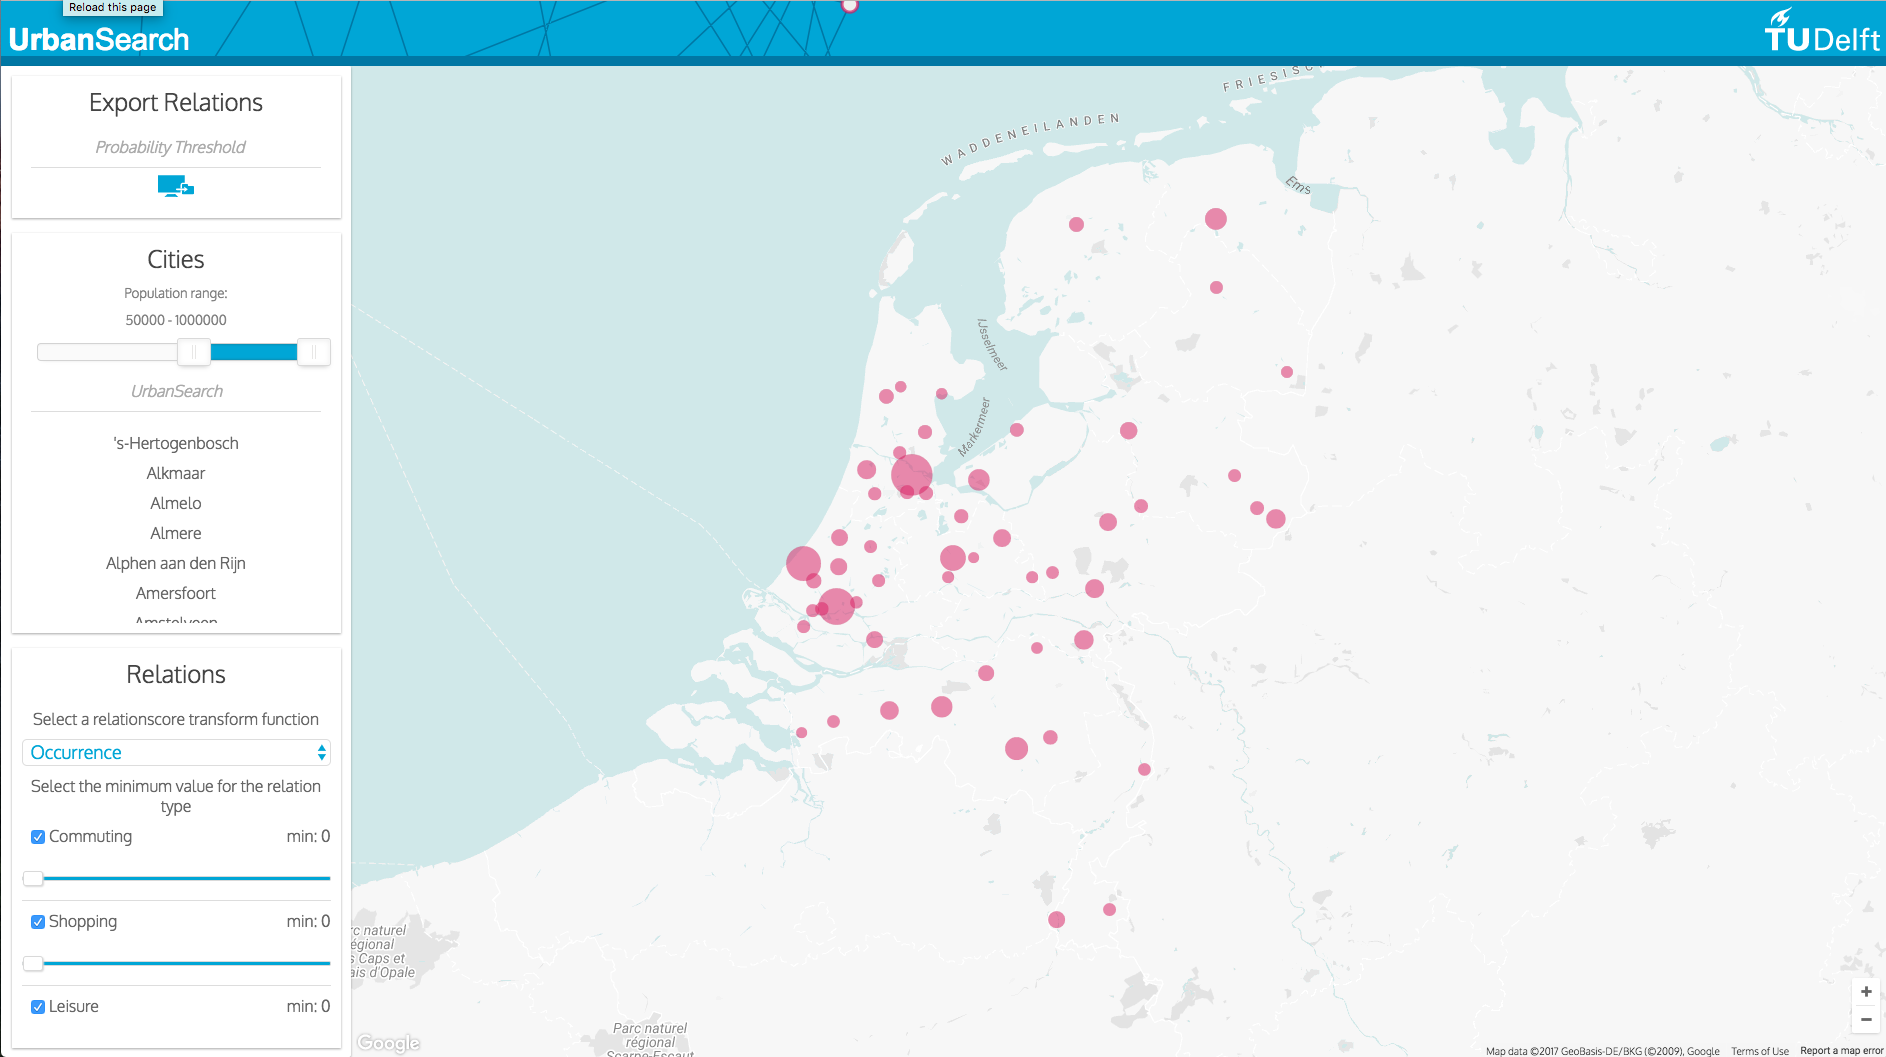
\includegraphics[width=.8\linewidth]{map.png}
    \caption{The interactive map with one relation selected}
    \label{fig:map}
\end{figure}

\subsection{Cities}\label{sec:city}
Cities are represented by circles which are drawn on the map and placed in the correct position using the latitude/longitude properties belonging to the city. We scale the circle based on the size of the population of the city. An example of a city on the map is show in figure \ref{fig:map-city}.

\begin{figure}[H]
  \centering
  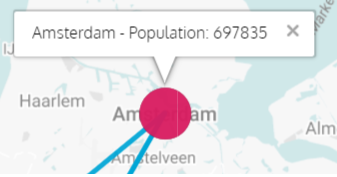
\includegraphics[width=.4\linewidth]{hover}
  \caption{Hovering over a city will display extra information about the city}
  \label{fig:map-city}
\end{figure}

When a user hovers over a city on the map, a pop up will appear with extra information about that city.\\
If a city is clicked the relations to other visible cities are shown. Clicking on a selected city toggles the visibility of the previously displayed relations. To make clear for the user  which cities are selected and which are not, we lower the opacity of selected cities.

\subsection{Relations}

Relations between cities are visualised using Google Maps Polylines\footnote{\url{https://developers.google.com/maps/documentation/javascript/3.exp/reference#Polyline}}. Relations for a particular city are shown when a city node is selected as described in \ref{sec:city}.\\
\begin{figure}[H]
  \centering
  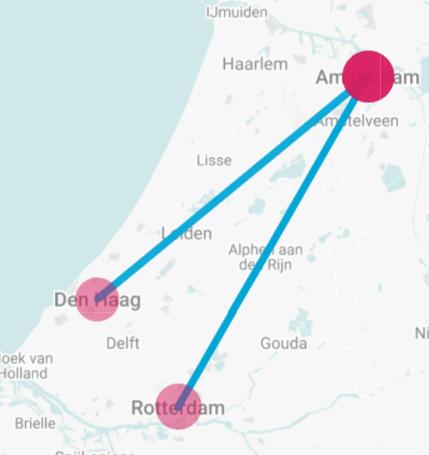
\includegraphics[width=.4\linewidth]{click}
  \caption{Selected city showing relations to other visible cities}
  \label{fig:sub2}
\end{figure}

Clicking on a relation opens up a new card containing information about this relation. The details about this card are discussed in \ref{sec:rel-info}.\\
The opacity of a relation indicates the relative strength of the relation compared to the relation with the highest score in the system. An example is given in figure \ref{}.

\begin{figure}[H]
  \centering
  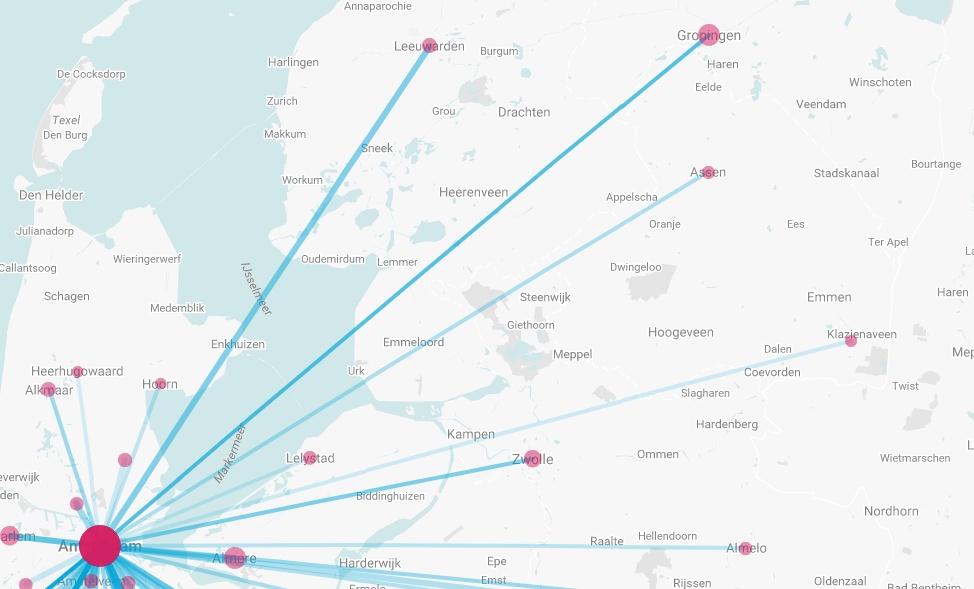
\includegraphics[width=.8\linewidth]{relation-opacity}
  \caption{A higher opacity indicates a weaker relative total strength of the relation. So Groningen has a stronger connection with Amsterdam then Assen.}
  \label{fig:relation-opacity}
\end{figure}


\subsection{Sidemenu}
The side-menu displayed in figure \ref{fig:sidemenu} allows the user to control the information that is displayed on the map. It is also the . The basic layout of the sidemenu is displayed in figure \ref{fig:sidemenu}. First we will discuss the elements that are always available in the sidemenu. Finally we will discuss dynamic content that can be added and removed from the sidemenu.

\begin{figure}[H]
    \centering
    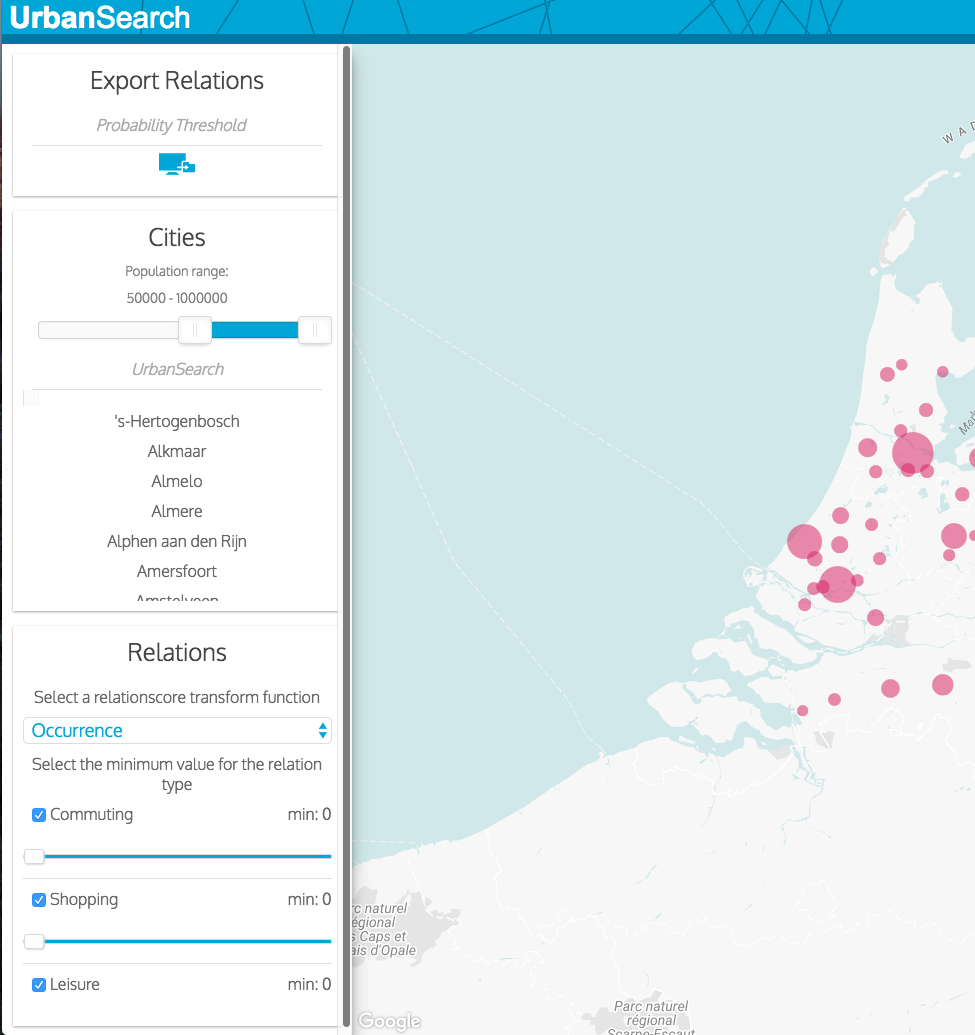
\includegraphics[width=.6\linewidth]{sidemenu}
    \caption{The sidemenu displayed on the left side of the interface}
    \label{fig:sidemenu}
\end{figure}


\subsubsection{City Controls}
The city controls displayed in figure \ref{fig:city-control} allow users to control the visibility of cities and city relations.\\
The population slider can be used to set the visibility of cities. All cities with a population size that is in the selected range are displayed on the map.\\
The search input allows the user to search a list of visible cities. When a city in the list is clicked, the relations for this city are shown on the map.

\begin{figure}[H]
    \centering
    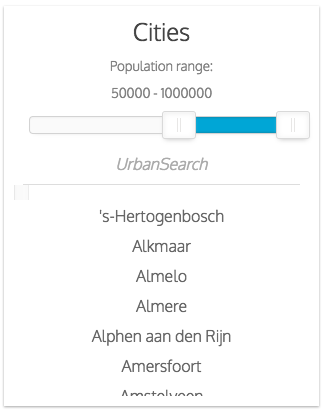
\includegraphics[width=.4\linewidth]{city-control}
    \caption{The city control card}
    \label{fig:city-control}
\end{figure}

\subsubsection{Relation Controls}
Using the relation controls displayed in figure \ref{fig:rel-control} an user can manipulate how intercity relations are displayed.\\
First of all the user can select several "transforms" from the drop-down that is available in the relation controls card. These transforms calculate a new value for the relation strengths based on the original values of the relations (which basically means the count of documents per category gets transformed for every relation). After the transform we get 


In the relations section of the menu a dropdown menu is displayed which is used to select how the weights of the relations should be calculated. The standard way is to just select the occurrences of documents per relation type. However it is also possible to use a gravity model, which takes the population and the distance between cities into account. \todo{can we do this?} Beneath that are sliders for the different relationship types. Here you can change the minimum occurrences a relation type should have per two cities before the relation is taken into account. There is also an option to turn off the relation types entirely.

\begin{figure}[H]
    \centering
    \includegraphics[width=.4\linewidth]{rel-control}
    \caption{Relations options}
    \label{fig:rel-control}
\end{figure}

\subsubsection{Export}
The first section on the menu is an export option. Here a button is displayed which can be used to export all relations between cities in an excel file (CSV). Above this button is a field in which a probably threshold can be set for the export. 

\begin{figure}[H]
    \centering
    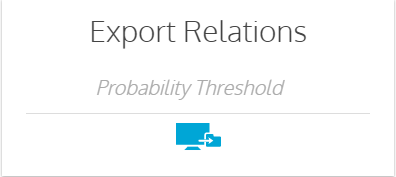
\includegraphics{export}
    \caption{Export}
    \label{fig:infoflow}
\end{figure}

\subsubsection{Relation Information}\label{sec:rel-info}
\subsubsection{Relation Documents}


\section{The Menu}
The menu on the left of the screen displays three different sections. The first section displays an option to export the data. The second section can be used to determine what cities should be displayed on the map. The last section displays the different relation types. The thresholds cities should have for each type can be adjusted here. This section also includes an option to select other weighting models that can be used.


\section{The Map}
After a few seconds needed to load the relations, a map should be displayed. This map first only contains some cities. The scroll wheel of the mouse or the plus and minus buttons in the lower right corner of the map for zooming. When hovering over a city with the mouse the population of that city will be displayed. To show the relations of a city, that city can be clicked on. The cities showing relations will have a slightly darker color than cities that have not been clicked on. You can also click on a relation. This will open up an extra window in the menu containing information about that relation.

\begin{figure}[H]
    \centering
    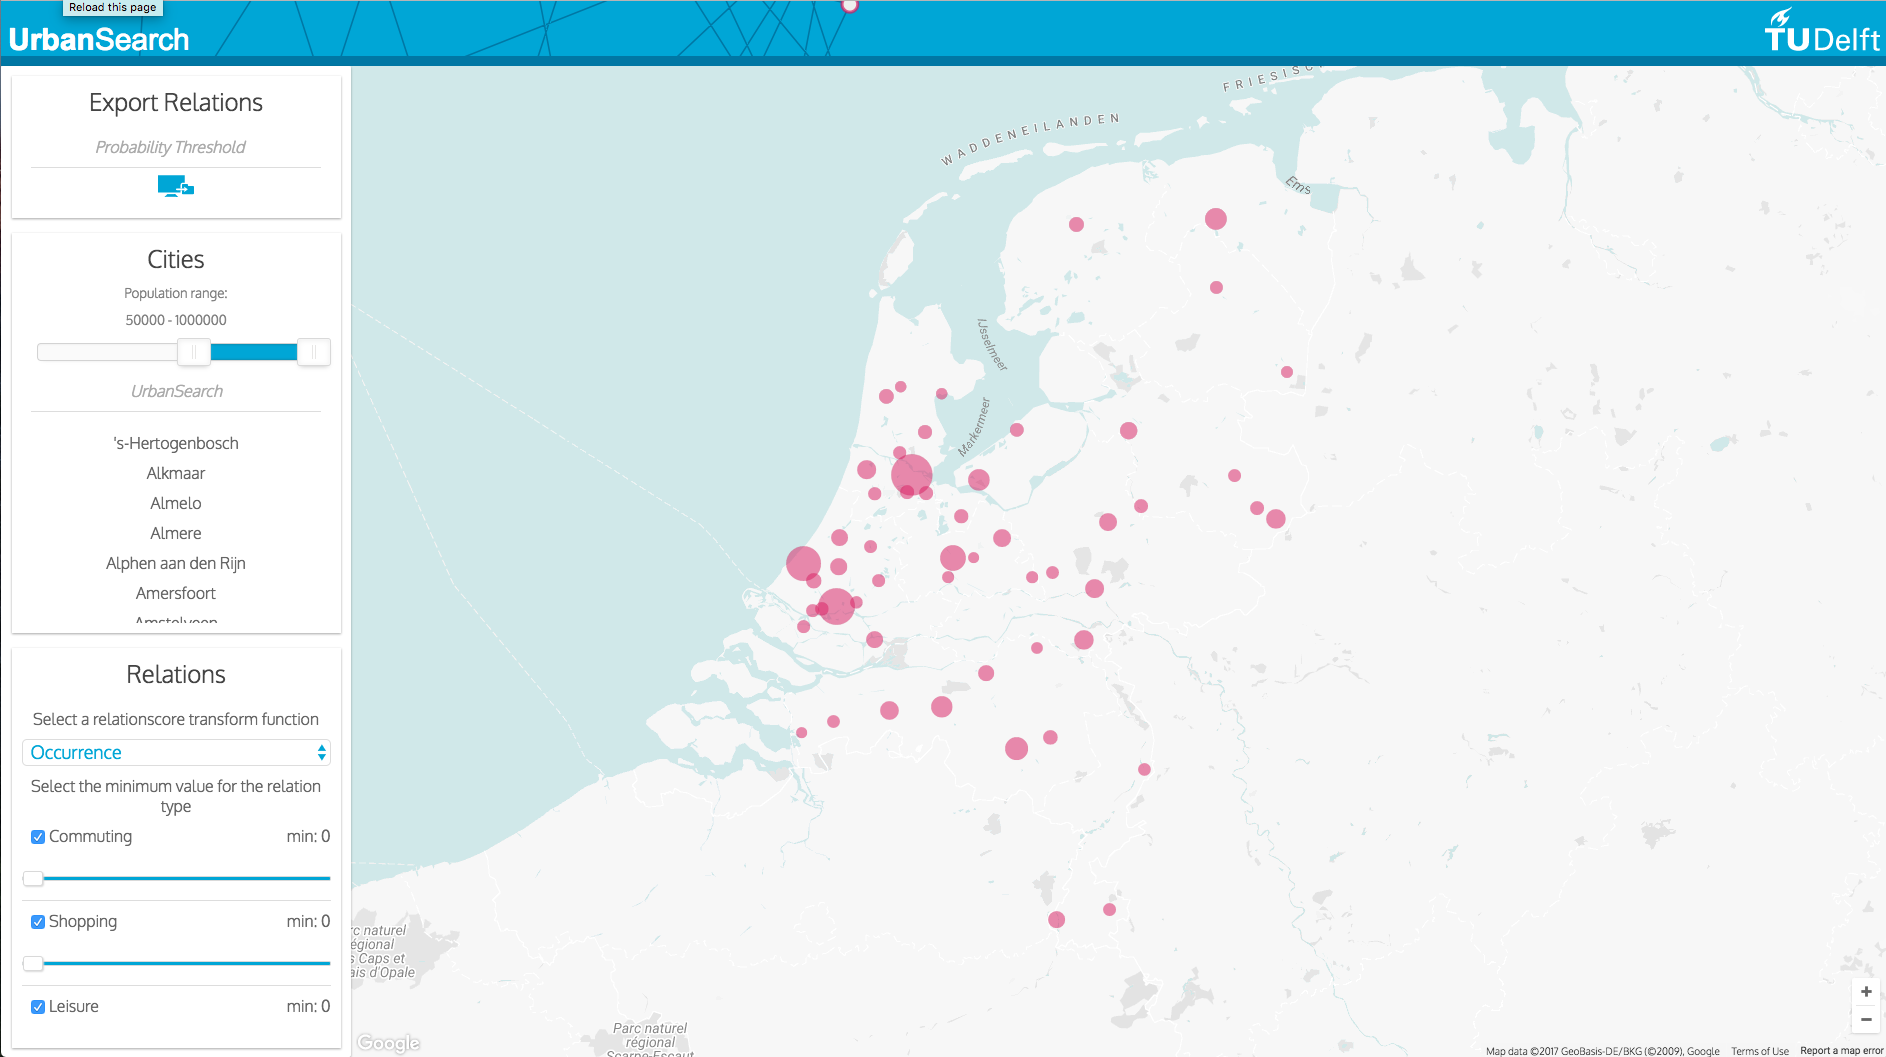
\includegraphics[scale=.5]{map}
    \caption{Map}
    \label{fig:infoflow}
\end{figure}





\subsection{Relation window}
When clicking on a relation an extra window in the menu will be opened. This contains all information about the relation between the two cities. The strength of the relations (amount of documents found for the relation between those cities) will be displayed, as well as the strength of the relations per relation type (such as commuting, shopping, leisure, ..). To check how these relationships were found the option on the lower end of this window  can be used to open up another window displaying all documents that connect those two cities.

\begin{figure}[H]
    \centering
    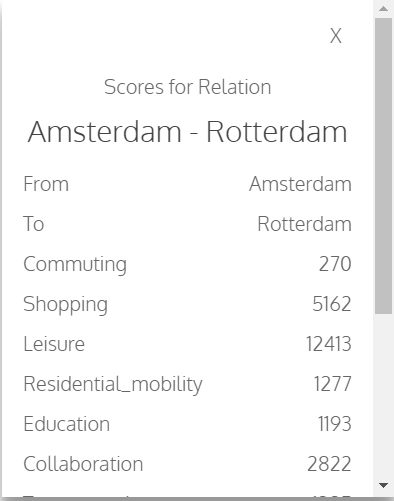
\includegraphics[scale=.7]{Score}
    \caption{Relations scores between two cities}
    \label{fig:infoflow}
\end{figure}


\subsection{Documents connecting two cities menu}
In this new window all documents will be displayed. For each document the type of relation to which the document fits and the probability this documents fits to that relation is displayed. If a document does not fit to the relation types (and is thus labelled other), it is not displayed here. The documents can be downloaded in a text file by clicking on them.

\begin{figure}[H]
    \centering
    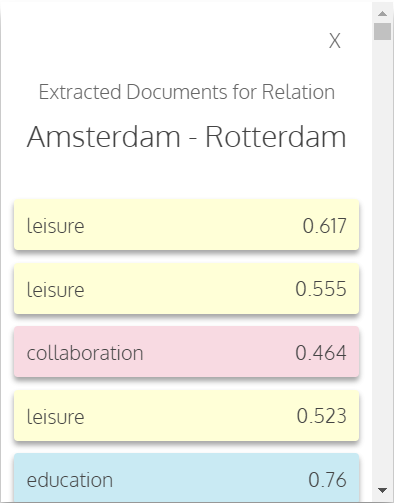
\includegraphics[scale=.7]{documents}
    \caption{Documents included in relations}
    \label{fig:infoflow}
\end{figure}

